\chapter{Implementation}
The implementation is divided into several modules: \textit{core} (code for computing different equilibria), \textit{web} (a backend engine that allows to play games and stores the results in a database), \textit{console} (a console client for the web API), \textit{structures} (common structures for \textit{web} and \textit{console}), and \textit{analysis} (Spark code to analyze large datasets of games).
Each module is described in a separate section below.

There are several services ready to be used via Docker Compose, and can simply be run without the need of installing any additional software:
\textit{web} (the web API server), \textit{postgres} (a PostgreSQL database; is started automatically when running \textit{web}), \textit{console} (the console interface), \textit{analysis} (Apache Spark with commands from the \textit{analysis} module made available), and \textit{sbt} (the building tool; can be used to compile modules or to run tests).

\section{Core Module}
While the core module does not contain much code, it is the heart of this project.
It defines the following entities:
\begin{itemize}
	\item \textsc{Game}: a case class that represents a game in normal form for two players.
	\item \textsc{BestResponse}: a trait that describes a best response, given a game and the opponent's strategy.
	It is implemented by the following objects:
	\begin{itemize}
		\item \textsc{NashianBestResponse}
		\item \textsc{PerfectlyTransparentBestResponse}
	\end{itemize}
	\item \textsc{GameGenerator}: an object for generating random games.
\end{itemize}

\section{Web Module}
\begin{figure}
	\hspace{-1cm}
	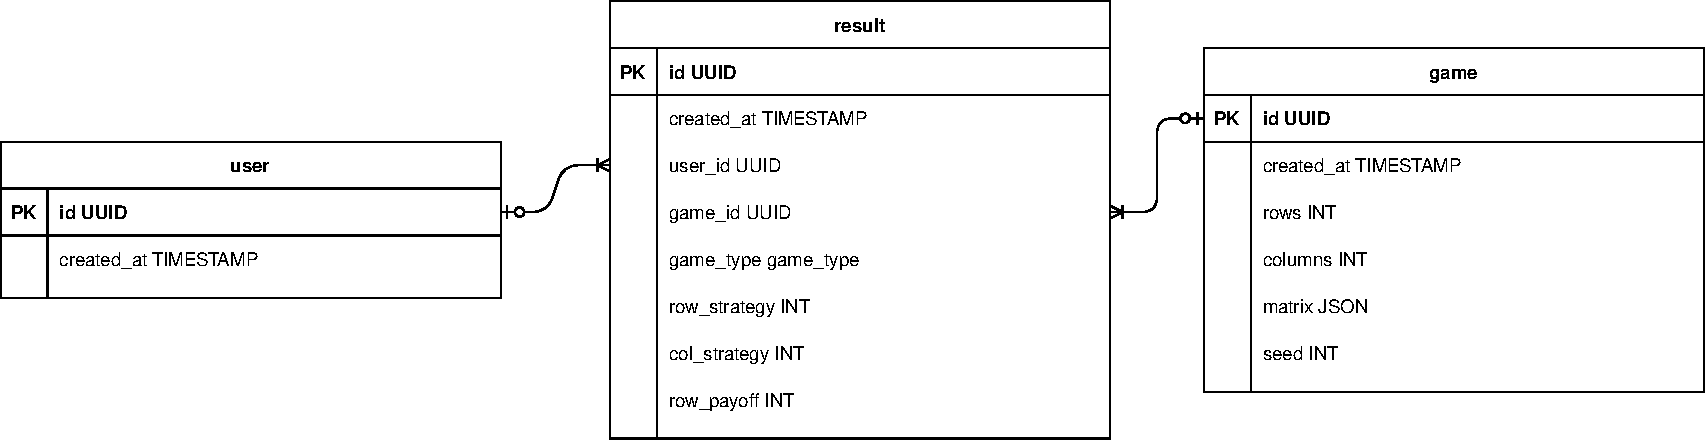
\includegraphics[width=14cm]{fig/schema.pdf}
\end{figure}

\section{Console Module}

\section{Analysis Module}
